\subsection{DIRC signal}

\begin{figure}[!h]
\centering
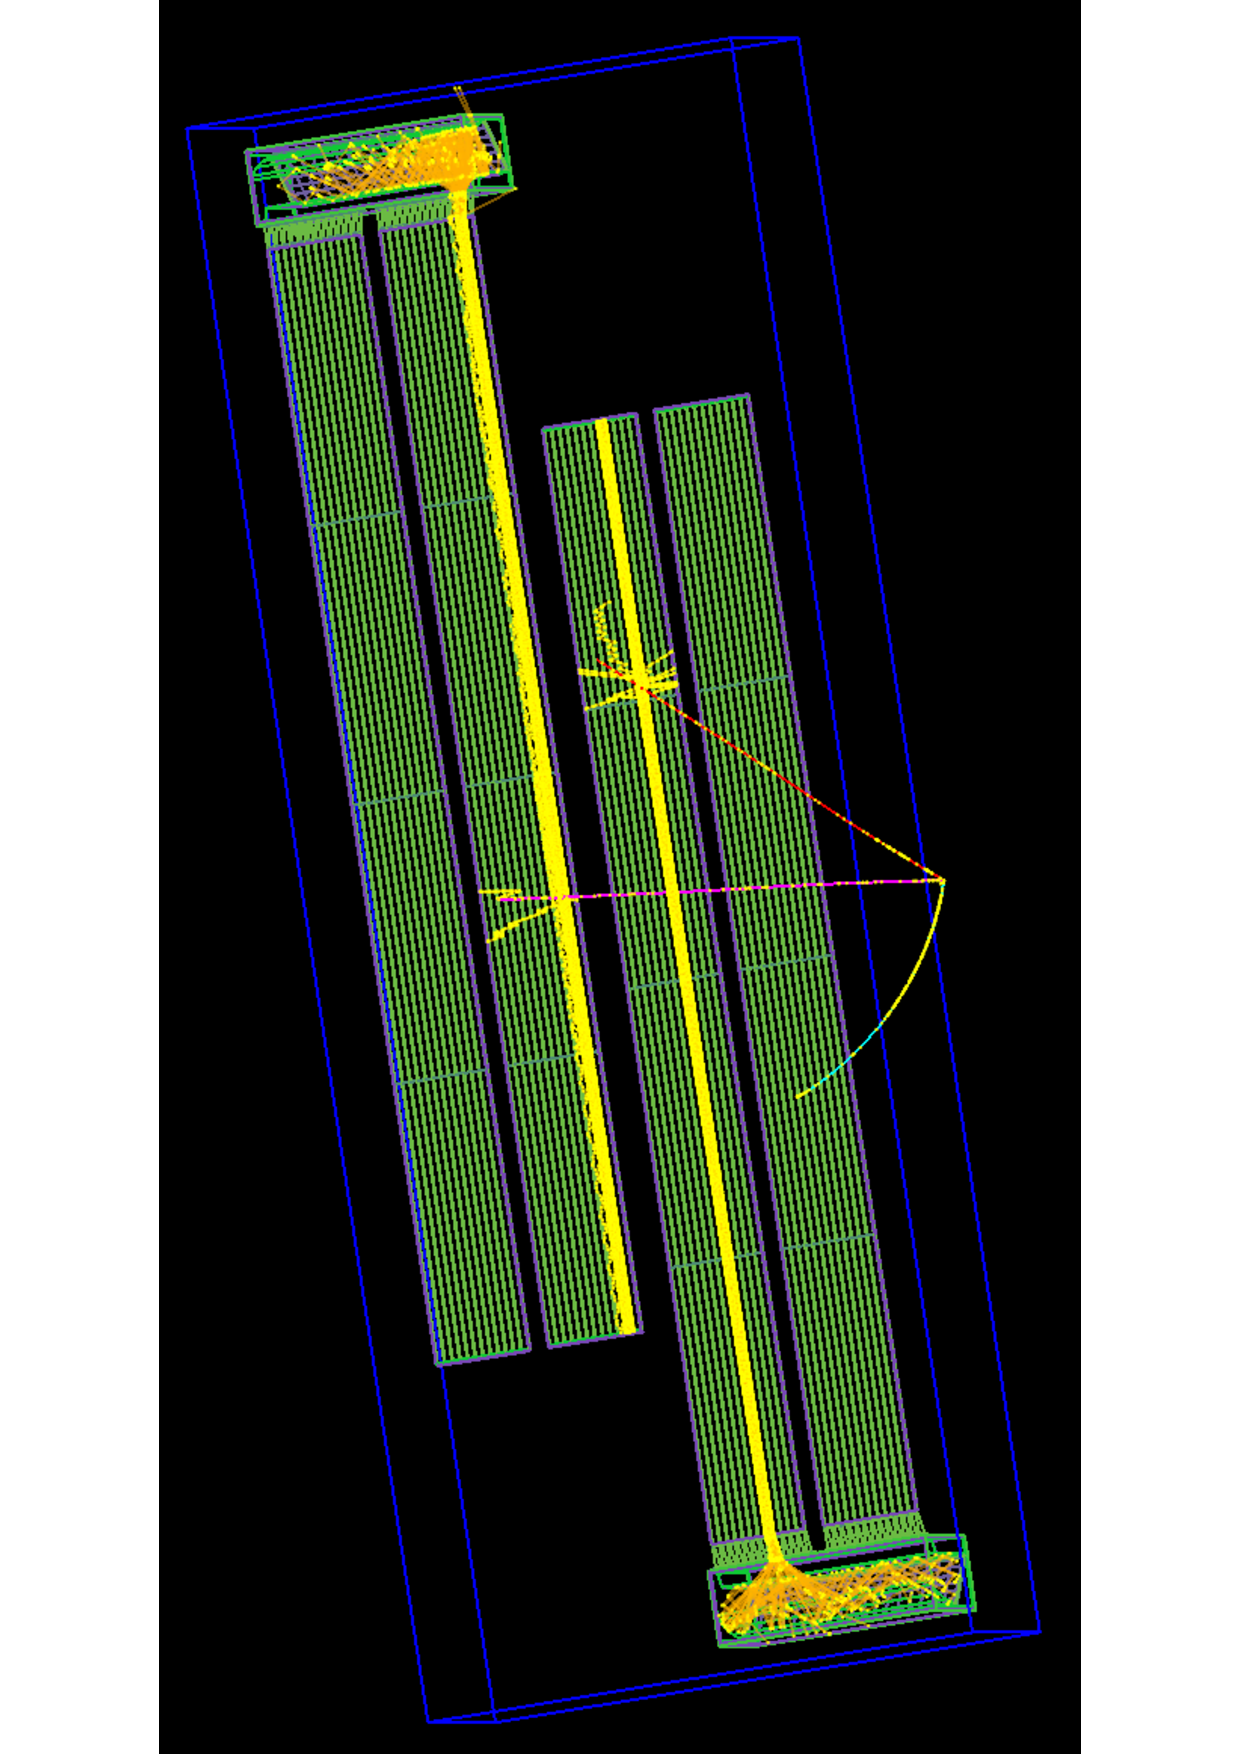
\includegraphics[angle=270,width=0.8\textwidth]{pics/eta2300decay.pdf}
\caption{\label{pic:eta2300}
An event showing the decay of $\eta(2300)$ into a kaon (red track) and a pion (magenta track). 
%A pion is shown in magenta, a kaon is shown in red. 
%A proton is shown in cyan. 
The pion and proton create Cherenkov photons (yellow tracks) inside two different DIRC radiators. The photons are transported to the optical boxes and imaged onto photodetection planes.
}
\end{figure}

Figure~\ref{pic:eta2300} shows a decay of $\eta(2300)$. The final state pion is shown in magenta and hits the upper bar box. The final state kaon is shown in red and hits the lower bar box. Both charged particles produce Cherenkov photons (their trajectories are shown in yellow), that propagate inside individual radiators towards the optical boxes, where they are detected. 
%An example of the single event hit pattern for a kaon and pion are shown in Fig.~\ref{pic:hitpat1} in the upper row. 

Typical GlueX DIRC hit patterns are shown in Fig.~\ref{pic:hitpat1}. DIRC does not try to reconstruct the shape of the hit pattern, but use different methods to compare hit patterns $(x,y,t)$\footnote{It is convenient to use a separate coordinate system on the photodetection plane. There $x$ axis goes along the long rows of PMTs containing $18$ sensors each, and $y$ axis goes along the short PMT rows of $6$ sensors each.} to expectations for different particle hypotheses ($e, \mu, \pi, K, p$).

\begin{figure}[!h]
\centering
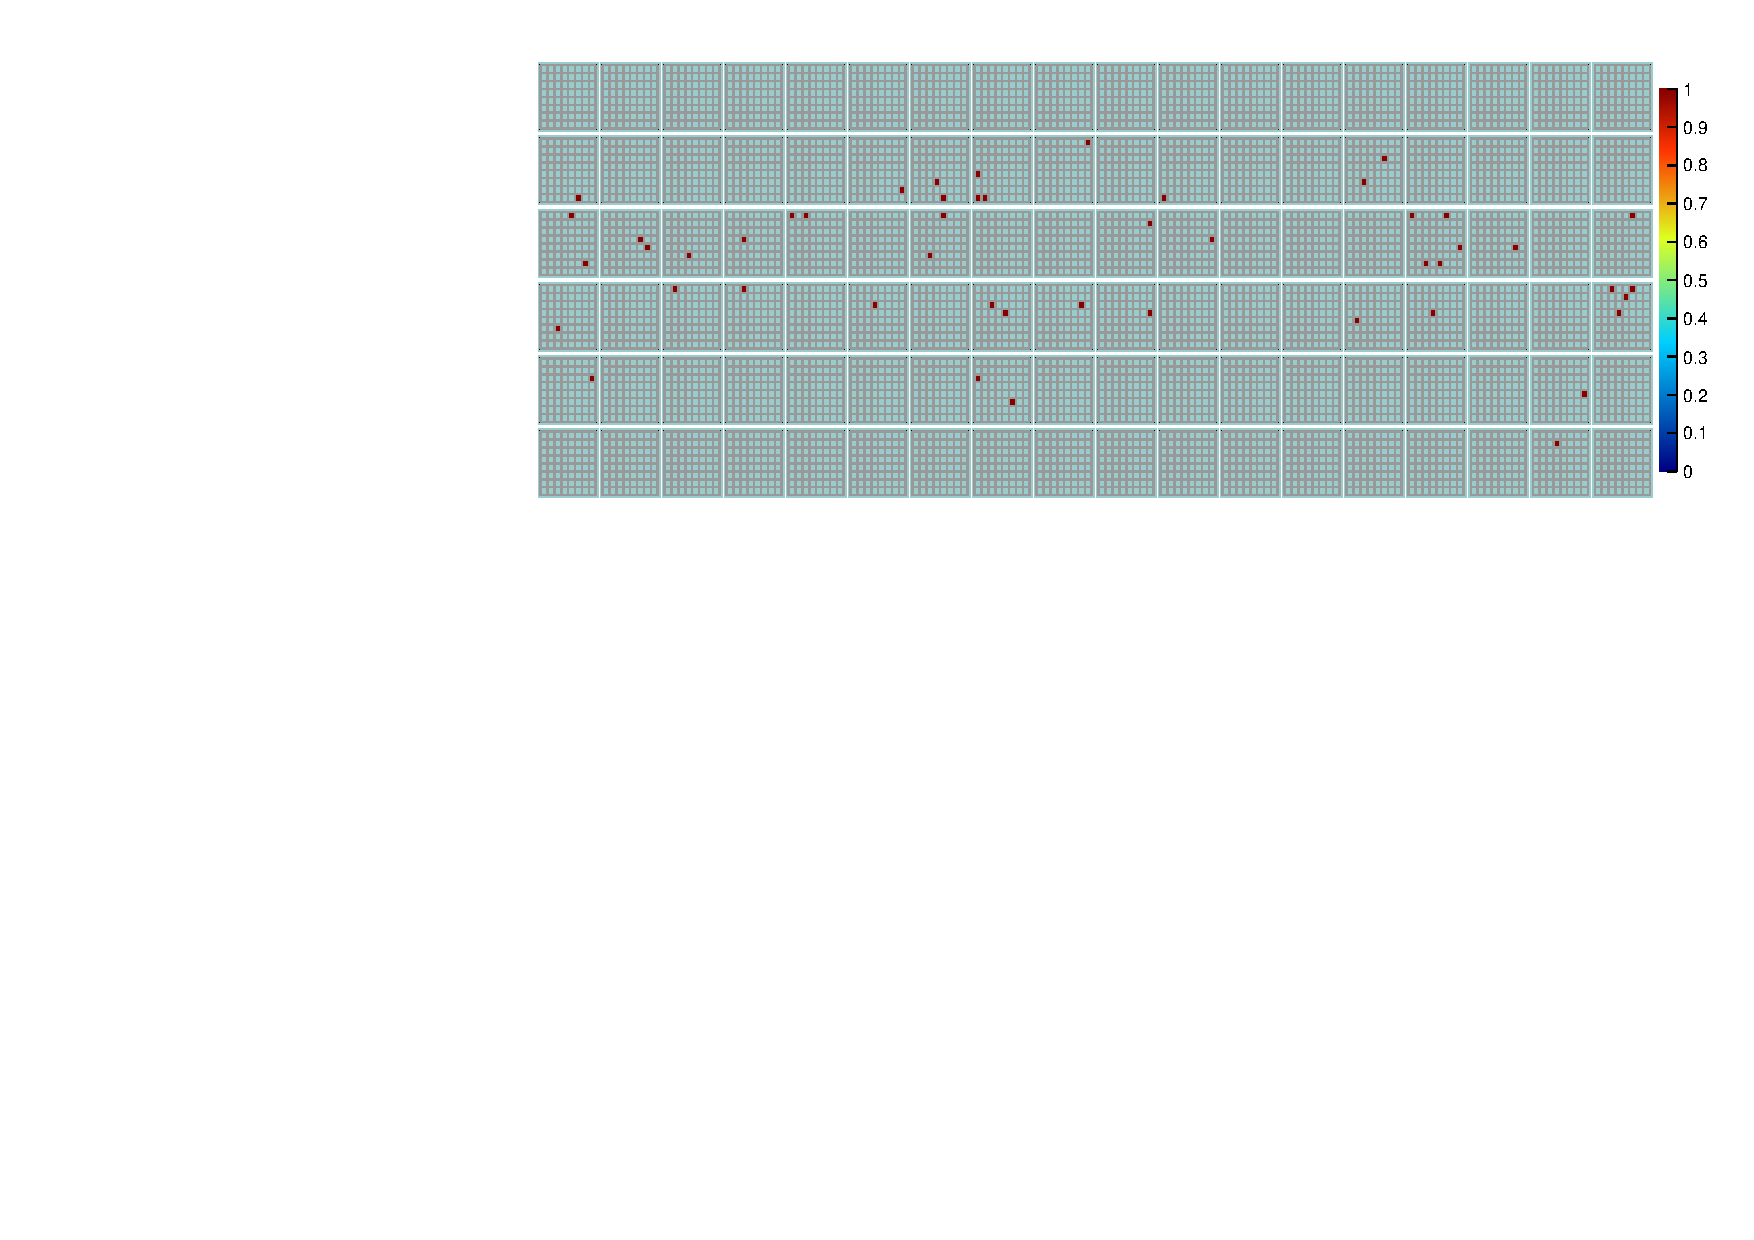
\includegraphics[angle=0,width=0.47\textwidth]{pics/single_ka_th8_phi158_p2.pdf} \hspace{0.5cm} 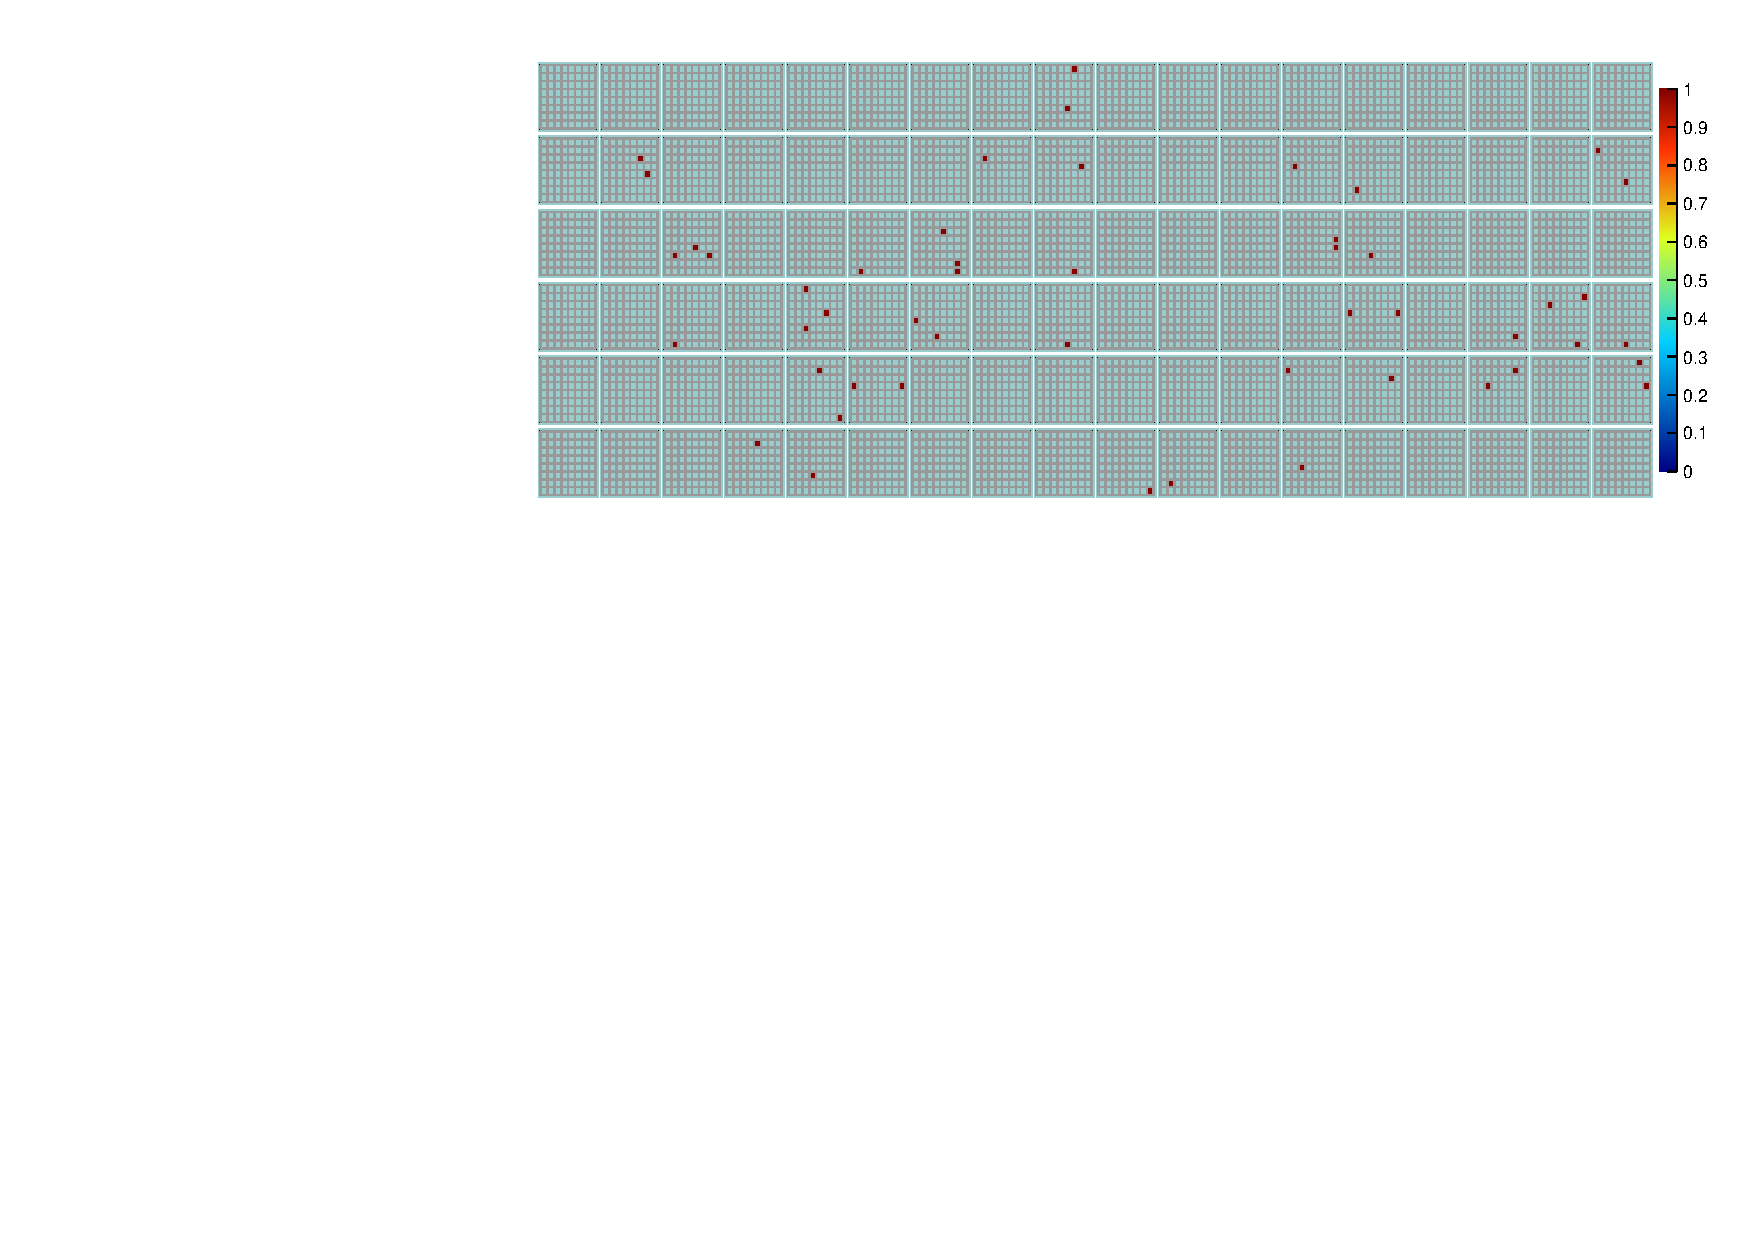
\includegraphics[angle=0,width=0.47\textwidth]{pics/single_pi_th8_phi158_p2.pdf}\\
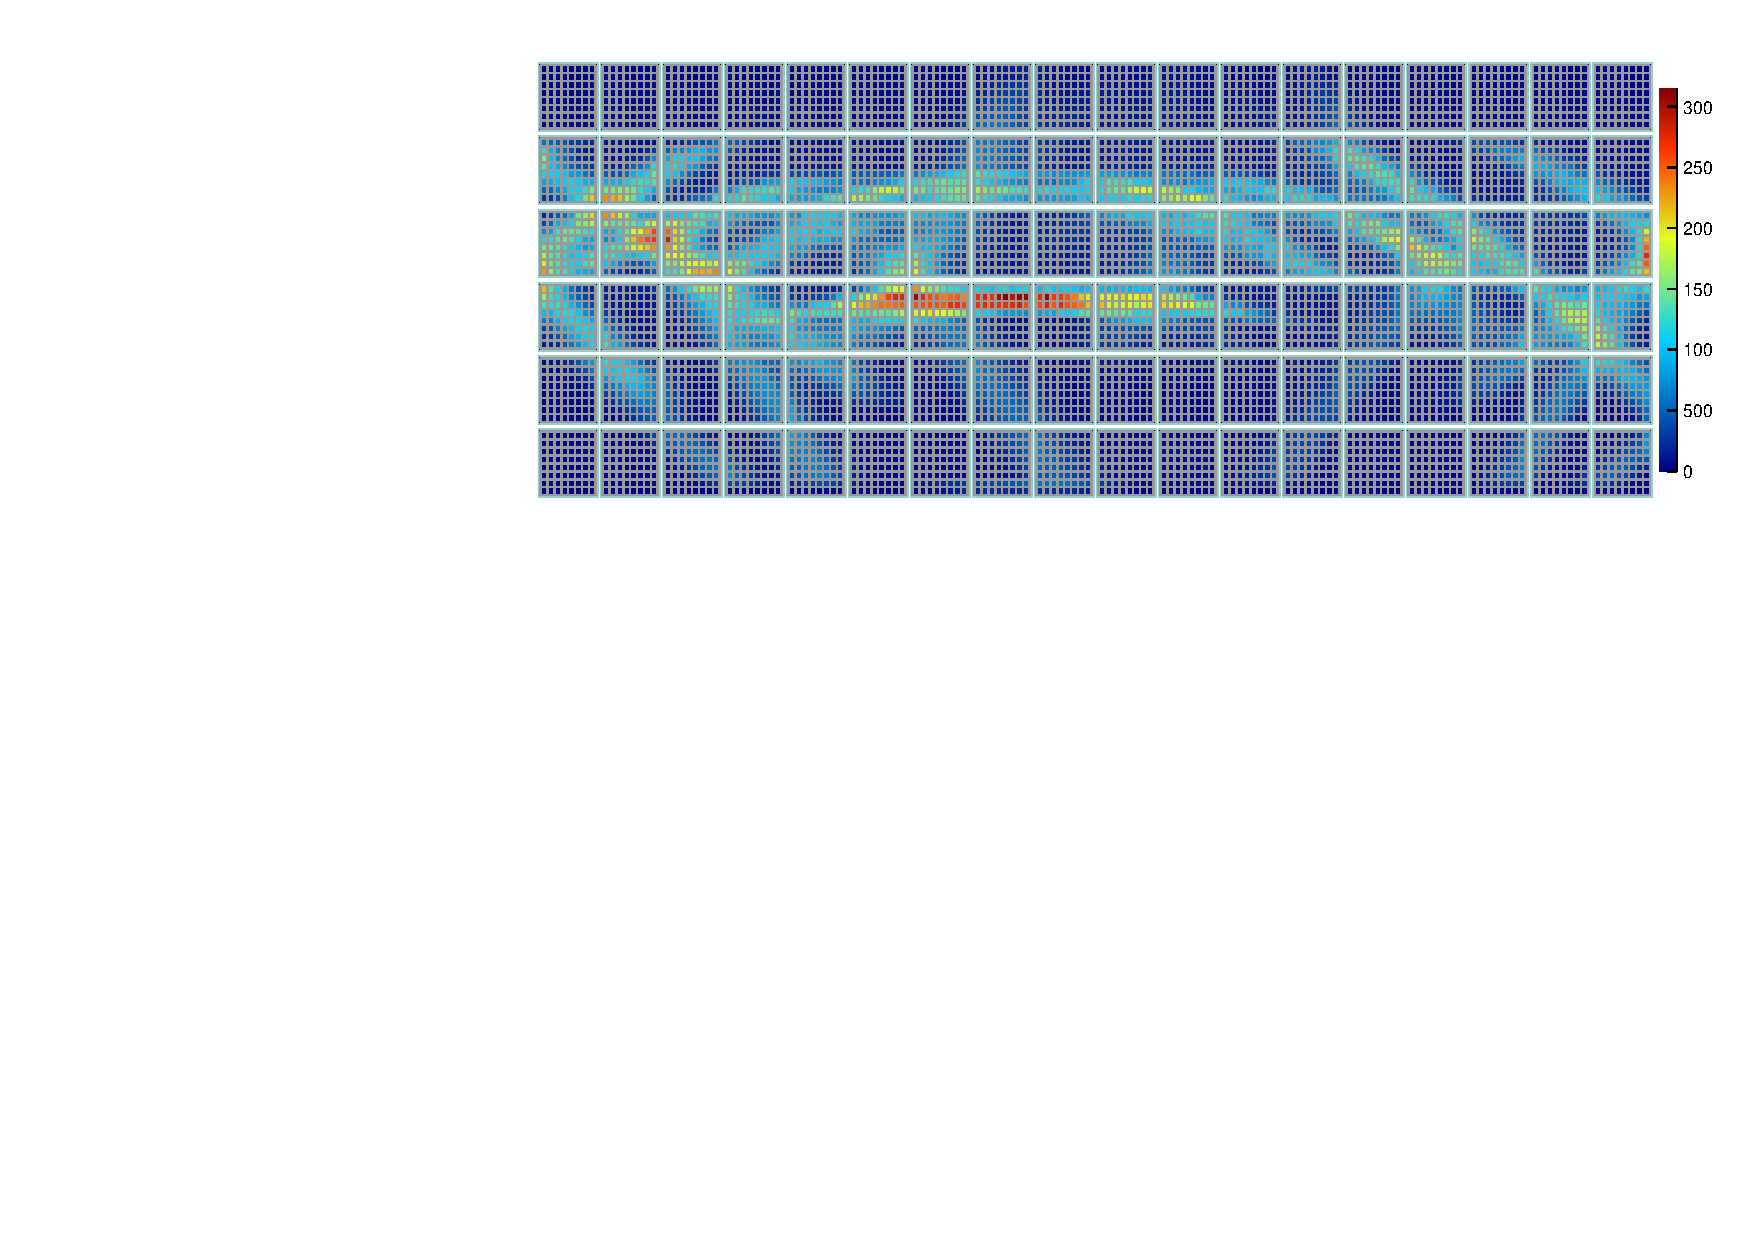
\includegraphics[angle=0,width=0.47\textwidth]{pics/ka_th8_phi158_p2.pdf} \hspace{0.5cm} 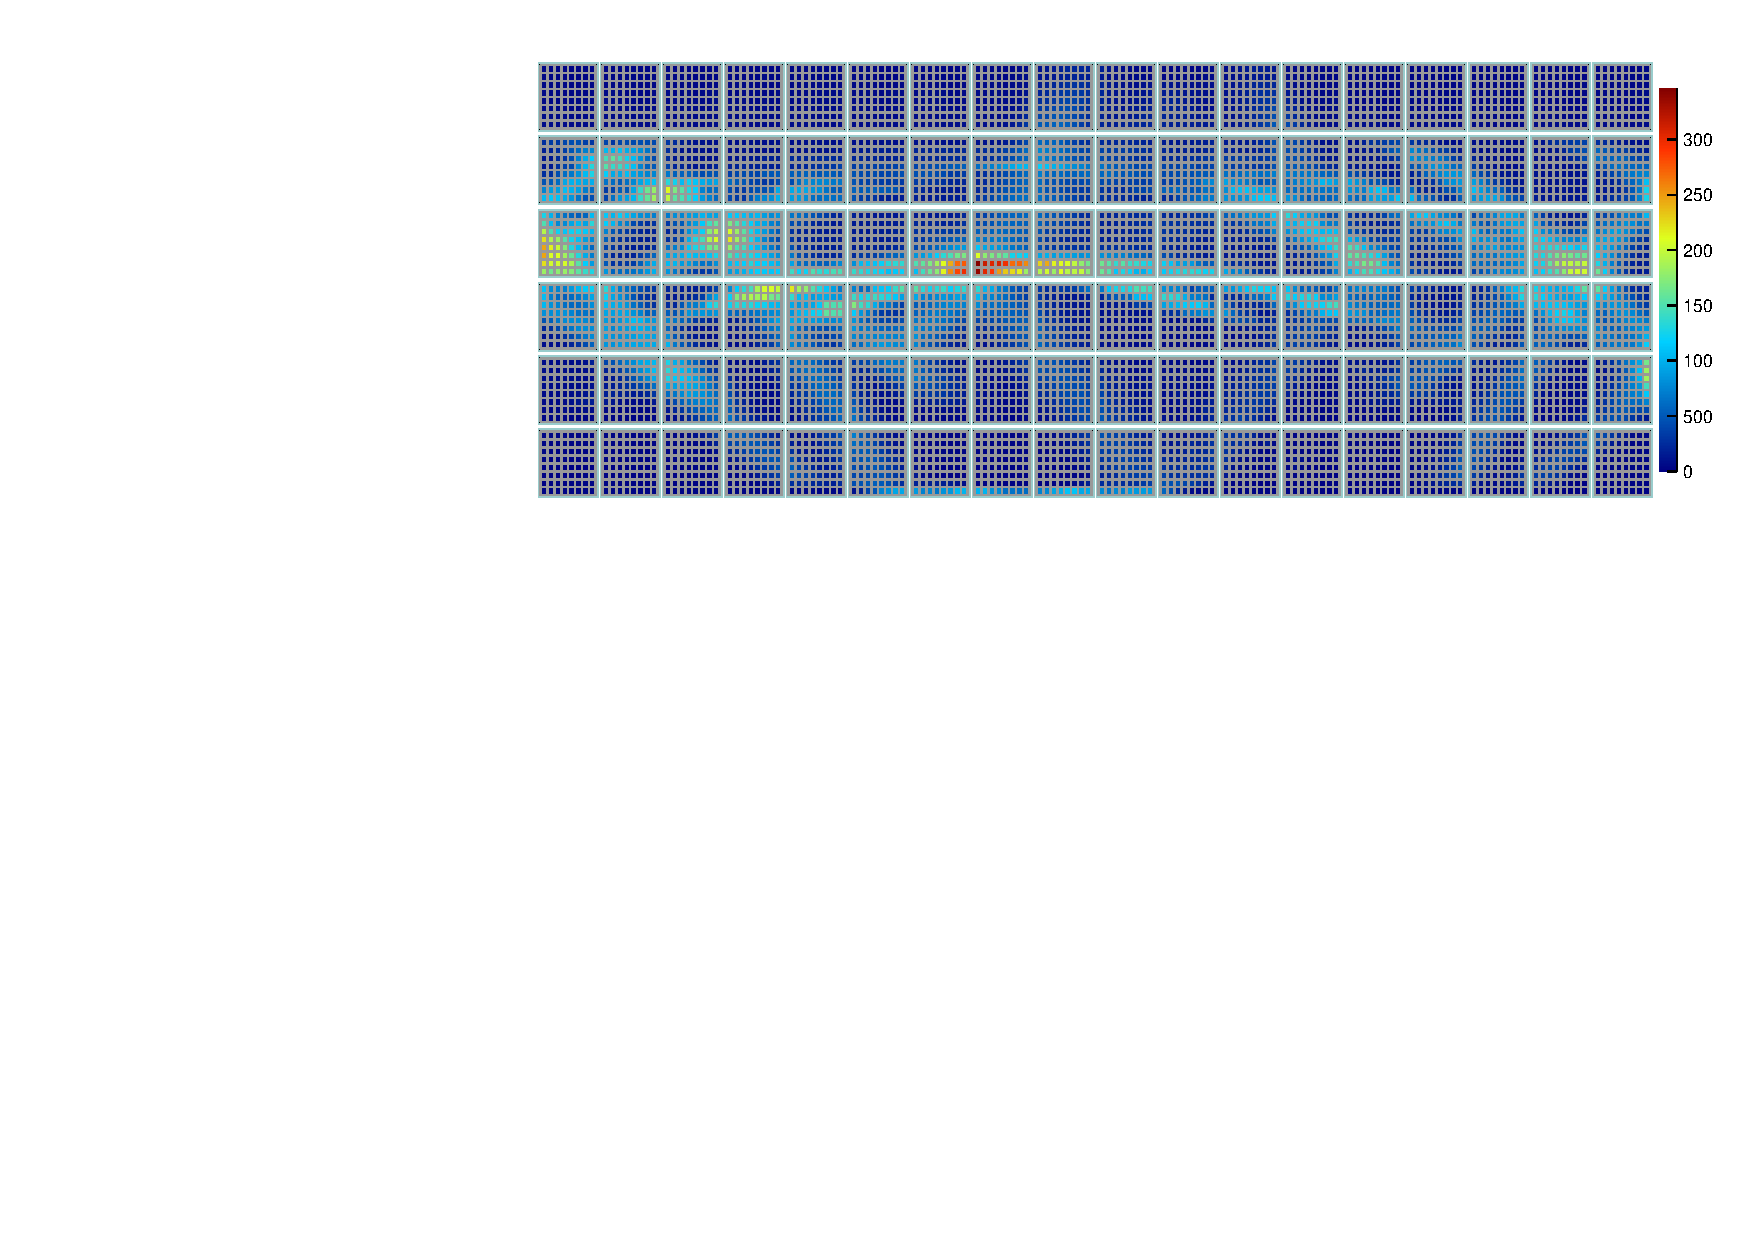
\includegraphics[angle=0,width=0.47\textwidth]{pics/pi_th8_phi158_p2.pdf}
\caption{\label{pic:hitpat1}
Typical GlueX DIRC hit patterns. The left column shows pions, and the right one -- kaons. Signals from single charged particles (upper row) look quite uncorrelated, and the cumulative patterns (bottom row) represent the complexity of the patterns. Samples of single kaons and pions with momentum of 2 GeV/c and direction defined by $\theta = 1.2^{\circ}$ and $\phi = 90^{\circ}$ angles were used to create these plots.
}
\end{figure}

\begin{figure}[!h]
\centering
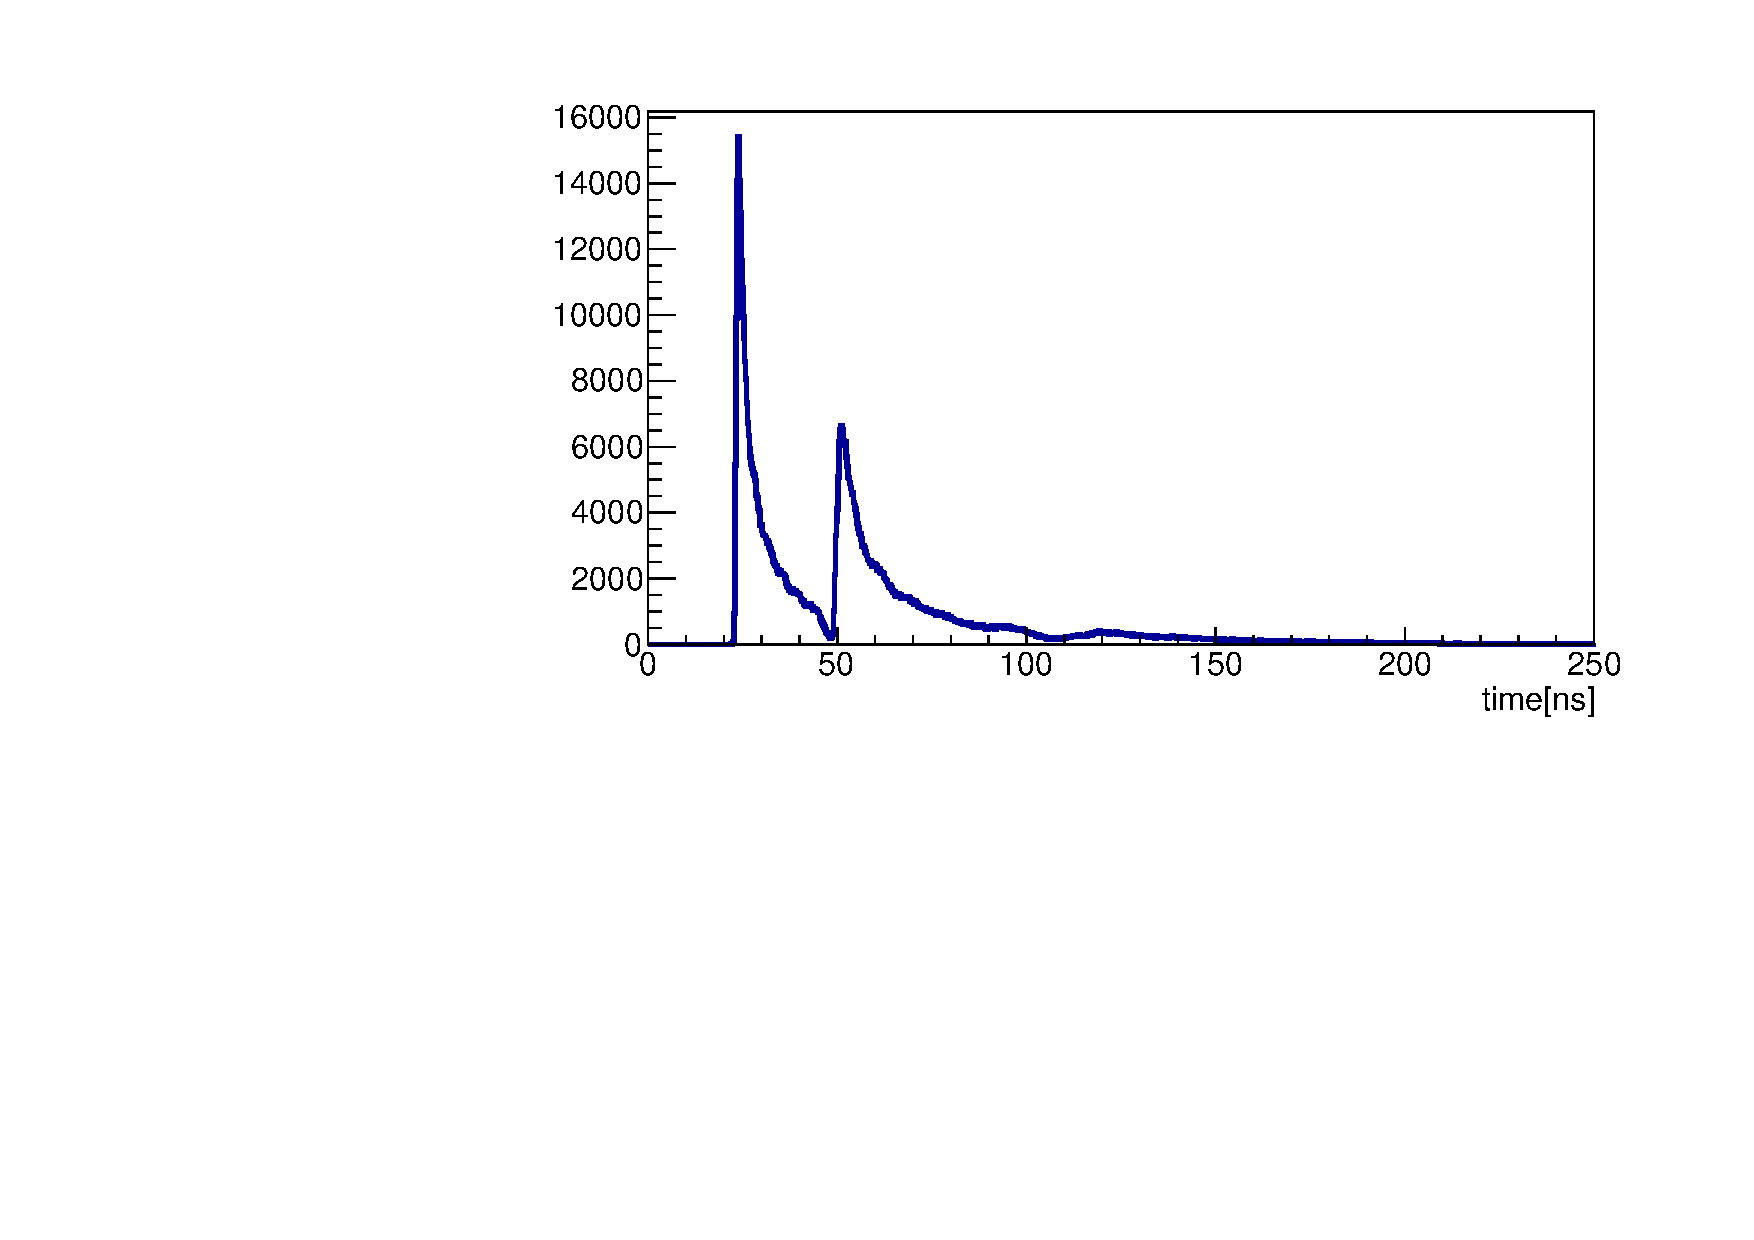
\includegraphics[angle=0,width=0.6\textwidth]{pics/Npho_th1_2_ph90.pdf}
\caption{\label{pic:time}
An example of the cumulative timing signal for charged kaons with momentum of 2 GeV/c and direction defined by $\theta = 1.2^{\circ}$ and $\phi = 90^{\circ}$ angles. The two peaks at $25$ ns and $55$ ns correspond to two groups of Cherenkov photons. The first group (left peak) contains direct photons, which were emitted towards the readout end of the bar unlike the second group (right peak), which first went to the mirror at the fught oton direction the particle dierend of the radiator, and then towards the optical box. The spread of the timing signal for one track is tens of nanoseconds. The dip in the spectra around $48$ ns show photon loss due to the total internal reflection inside the radiator. 
}
\end{figure}

DIRC measures $(x,y,t)$ of each detected Cherenkov photon. In $(x,y)$ the cumulative hit patterns look like conic sections with additional reflections (see cumulative hit patterns for different charged particle configurations \url{http://web-docs.gsi.de/~rdzhigad/www/research/hit-pattern-vs-theta-phi}). In the coordinate space ($x ,y$) some parts overlap, but timing helps to separate them.
An example of the cumulative timing spectra for charged kaons with fixed momentum and direction is shown in Fig.~\ref{pic:time}. 

%The ring image of the GlueX DIRC is a complicated pattern in $(x, y, t)$ space, which besides Cherenkov angle depends strongly on the particle impact position and the particle direction with respect to the sides of the quartz bar. For the forward GlueX DIRC geometry, the charged particle direction with respect to the sides of the DIRC radiators correlates with the position where the charged particle hit the DIRC wall. 

%An essential input for the DIRC reconstruction is the tracking information about the momentum of the charged particle and coordinate, where it hit the DIRC wall.

%To get a feeling about which parts of the photodetection plane are occupied more, and which less, we can have a look at the cumulative kaon occupancies originating from some relevant physics reactions or from general kaon background. Figure~\ref{pic:phi} shows an example for the cumulative kaon hit pattern for the decay of $phi_{1850}$. Kaon hit patterns for other reactions of interest and general background look very similar. The highest occupancy is around the third PMT row from the top. The hit pattern is not left-right symmetrical, as the left side of the optical box is closer to the beam line. The upper row of PMTs has the lowest occupancy. The simulation studies showed that removing this row does not impact to the detector performance in terms of photon yield and separation between pions and kaons (see Fig.~\ref{pic:5rows}).